\documentclass[tikz,svgnames]{standalone}

\usetikzlibrary{patterns}

\begin{document}
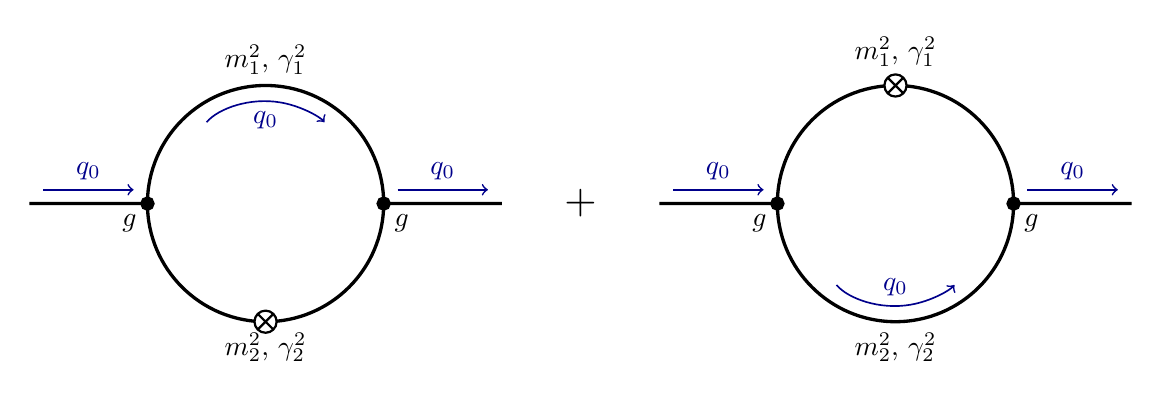
\begin{tikzpicture}[
    very thick,
    q0/.style={->,DarkBlue,semithick,yshift=5pt,shorten >=5pt,shorten <=5pt},
    cross/.style={
        path picture={
            \draw[black,thick]
            (path picture bounding box.south east) -- (path picture bounding box.north west)
            (path picture bounding box.south west) -- (path picture bounding box.north east);
          }
      }
  ]

  % Loop
  \def\radius{1.5}
  \draw (0,0) circle (\radius);
  \node[above] (1) at (0,\radius) {$m_1^2$, $\gamma_1^2$};
  \node[below] (2) at (0,-\radius) {$m_2^2$, $\gamma_2^2$};
  \draw[q0] (140:0.75*\radius) arc (140:40:0.75*\radius) node[midway,below] {$q_0$};
  \draw[fill=white,cross,thick] (0,-\radius) circle (4pt);

  % External lines
  \filldraw
  (-2*\radius,0) -- (-\radius,0) circle (2pt) node[below left] {$g$}
  (\radius,0) circle (2pt) node[below right] {$g$} -- (2*\radius,0);
  \draw[q0] (-2*\radius,0) -- (-\radius,0) node[midway,above] {$q_0$};
  \draw[q0] (\radius,0) -- (2*\radius,0) node[midway,above] {$q_0$};

  \node[xshift=4cm,scale=1.5] at (0,0) {$+$};

  \begin{scope}[xshift=8cm]
    % Loop
    \def\radius{1.5}
    \draw (0,0) circle (\radius);
    \node[above=3pt] (1) at (0,\radius) {$m_1^2$, $\gamma_1^2$};
    \node[below] (2) at (0,-\radius) {$m_2^2$, $\gamma_2^2$};
    \draw[q0,yshift=-10pt] (220:0.75*\radius) arc (220:320:0.75*\radius) node[midway,above] {$q_0$};
    \draw[fill=white,cross,thick] (0,\radius) circle (4pt);

    % External lines
    \filldraw
    (-2*\radius,0) -- (-\radius,0) circle (2pt) node[below left] {$g$}
    (\radius,0) circle (2pt) node[below right] {$g$} -- (2*\radius,0);
    \draw[q0] (-2*\radius,0) -- (-\radius,0) node[midway,above] {$q_0$};
    \draw[q0] (\radius,0) -- (2*\radius,0) node[midway,above] {$q_0$};
  \end{scope}

\end{tikzpicture}
\end{document}
